\documentclass[11pt]{article}


\usepackage{fullpage}
\usepackage{graphicx}
\usepackage{amsmath}
\usepackage{amssymb}
\usepackage{amsthm}
\usepackage{fancyvrb}

\newcommand{\myname}{Mehshan Mustafa}

\newenvironment{theorem}[2][Theorem]{\begin{trivlist}
\item[\hskip \labelsep {\bfseries #1}\hskip \labelsep {\bfseries #2.}]}{\end{trivlist}}
\newenvironment{lemma}[2][Lemma]{\begin{trivlist}
\item[\hskip \labelsep {\bfseries #1}\hskip \labelsep {\bfseries #2.}]}{\end{trivlist}}
\newenvironment{exercise}[2][Exercise]{\begin{trivlist}
\item[\hskip \labelsep {\bfseries #1}\hskip \labelsep {\bfseries #2.}]}{\end{trivlist}}
\newenvironment{problem}[2][Problem]{\begin{trivlist}
\item[\hskip \labelsep {\bfseries #1}\hskip \labelsep {\bfseries #2.}]}{\end{trivlist}}
\newenvironment{question}[2][Question]{\begin{trivlist}
\item[\hskip \labelsep {\bfseries #1}\hskip \labelsep {\bfseries #2.}]}{\end{trivlist}}
\newenvironment{corollary}[2][Corollary]{\begin{trivlist}
\item[\hskip \labelsep {\bfseries #1}\hskip \labelsep {\bfseries #2.}]}{\end{trivlist}}
\newenvironment{solution}{\begin{proof}[Solution]}{\end{proof}}
\newenvironment{idea}[2][Proof Idea.]{\textit{#1} #2}



\parindent0in
\pagestyle{plain}
\thispagestyle{plain}

\newcommand{\dated}{\today}

\begin{document}

\textbf{Introduction to the Theory of
Computation}\hfill\textbf{\myname}\\[0.01in]
\textbf{Chapter 2: Context-Free Languages}\hfill\textbf{\dated}\\
\smallskip\hrule\bigskip

\begin{problem}{2.22}
Let $C = \{x \# y \ | \ x, \ y \in \{0,1\}^{*} \ and \ x \neq y \}$. Show that $C$ is a context-free language.
\end{problem}

\begin{idea}[Informal description.]
A PDA can be constructed to recognize $C$ as follows:
\begin{enumerate}
\item Repeatedly compare each symbol $x_{i}$ of the string $x$ with the corresponding symbol $y_{i}$ of the string $y$. Accept, if $x_{i} \neq y_{i}$, or $y_{i}$ does not exist, which means that $|x| > |y|$.
\item Also accept, if $|x| < |y|$.
\end{enumerate}
\end{idea}

\begin{proof}
To show that $C$ is a context-free language, give state diagram of a PDA $P$ that recognizes $C$.
\begin{center}
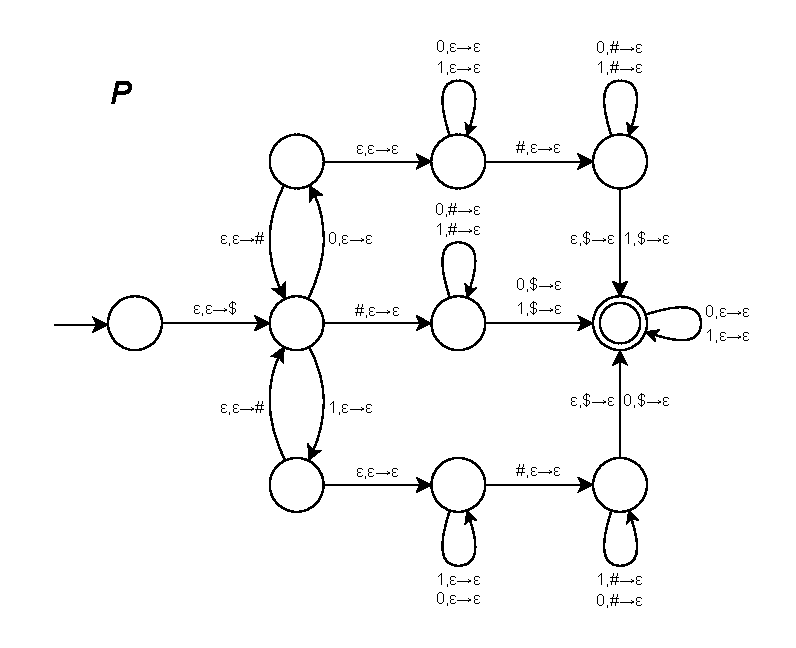
\includegraphics[scale=1.0]{Figures/Problem2.22.pdf} \\
State diagram of a PDA $P$ that recognizes $C$. Each time $P$ reads a symbol $x_{i}$, it non-deterministically compares it with $y_{i}$ and writes a $\#$ on the stack. This way, the PDA $P$ tracks the number of $x_{i}$'s read and compared.
\end{center}
\end{proof}

\end{document}
